\section{Deriving Electromagnetic Waves}

\begin{comment}
This lab steps studets through a derivation of electromagnetic waves, starting from how Maxwell fixed up Ampere's law, and culminating in his discovery that the speed of electromagnetic waves is the same as light.

Activity 1 points out that Ampere's law is missing something, which is qualitatively the displacement current.
Activity 2 steps them through the math leading to the constant mu_0 epsilon_0.
Activity 3 derives coupled differential equations, and then separates them into the wave equations for E and B.
Activity 4 has them calculate the speed of an electromagnetic wave from mu_0 and epsilon_0, and has them discover that it's the speed of light.  Wahoo!!!

I ran parts 2 and 3 as separate worksheets in spring 2015, and they worked well.  Students were able to crank through the math and physics okay (with occasional help an gentle nudges, as always).  

I started with the material from Activity 1 as a lecture before giving them the worksheets, and I essentially did activity 4 at the board too, having them calculate a number for the speed. I emphasized what a badass Maxwell had to be to pull this off.  In the end, they genuinely seemed excited to have figured out that light is an electromagnetic wave!  The one thing I'm not sure about is whether having the material in activities 1 and 4 as an interactive lab will be as engaging as the story I told at the board.  
--Matt Trawick, 6/2015

\end{comment}

Name \rule{2.0in}{0.1pt}\hfill{}Section \rule{1.0in}{0.1pt}\hfill{}Date
\rule{1.0in}{0.1pt}

\vspace{0.1in}
\textbf{Objective} 

In this lab, you will work through the logic that James Clerk Maxwell used to derive the properties of electromagnetic waves.  You'll start with a brief review of the laws of electricity and magnetism that you already know, and then you'll extend them slightly to discover something totally new and amazing!

\textbf{Activity 1: What's Wrong with Amp\`ere's Law?}

(a) You have already learned that Amp\'ere's law, $\oint \vec B \cdot \vec{ds} = \mu_0I_{enc}$, can be used to help you calculate the magnetic field near wires carrying electric current.  In the figure below, what is the direction of the magnetic field at the point shown, just above the current carrying wire?

\begin{center}
    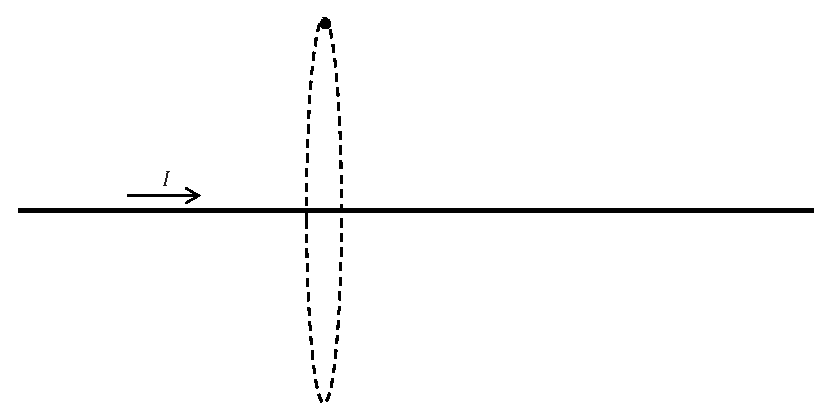
\includegraphics[width=0.4\textwidth]{deriving_em_waves/wire_and_loop.eps}
\end{center}

In the 1850s, Amp\'ere's law was well understood.  But a very clever Scotsman named James Clerk Maxwell realized there might be something wrong with it.  He thought of the example shown below, in which current through a wire is charging up a capacitor.
\begin{center}
    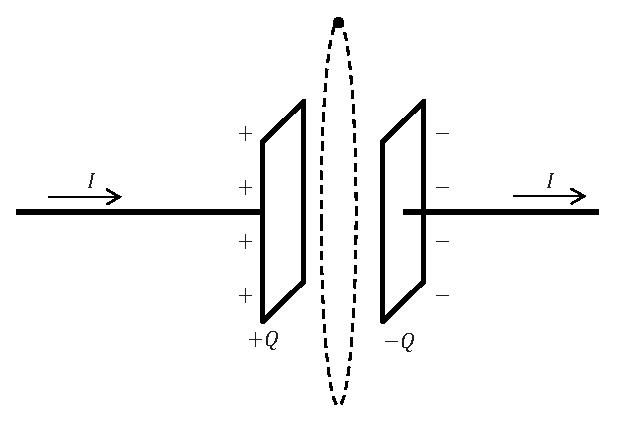
\includegraphics[width=0.4\textwidth]{deriving_em_waves/capacitor_and_loop.eps}
\end{center}

(b) Suppose you draw the circular path for Amp\`ere's law (the ``Amperian loop'') around the gap between the two capacitor plates as shown above.  Is there any actual current flowing between the two plates that is ``enclosed'' by that loop?   
\vspace{0.5in}

(c) According to a straightforward interpretation of $\oint \vec B \cdot \vec{ds} = \mu_0I_{enc}$, what is the magnetic field at the point shown in the figure above?  
\vspace{0.5in}

%\pagebreak
(d) Ampere's law, as we've written it so far, seems to imply that the magnetic field above the wire can change discontinuously to zero if you move by even one \textit{nanometer} to the right, depending on whether your loop is just to the left or just to the right of the capacitor plate.  Does it seem plausible to you that the magnetic field would change discontinuously like that?
\vspace{0.5in}

(e)  There's another, more sophisticated argument against the magnetic field going to zero that's based on a mathematical idea known as Stoke's Theorem.  When we say ``current enclosed by a loop,'' what we really mean is ``current going through a surface bound by a loop.'' But there's nothing that says that the surface has to be flat, or even that the loop has to lie in a plane.  In the drawings below, do the two surfaces both have the same current flowing through them?
\begin{center}
\vspace{-0.1in}
    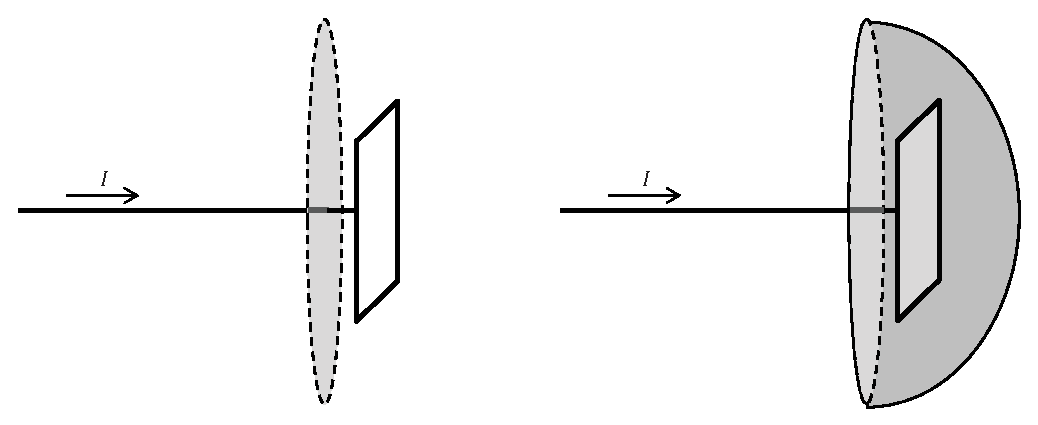
\includegraphics[width=0.5\textwidth]{deriving_em_waves/two_surfaces.eps}
\vspace{-0.1in}
\end{center}

So according to $\oint \vec B \cdot \vec{ds} = \mu_0I_{enc}$, the magnetic field B at a point near a wire can change from zero to nonzero by either moving the point to the left or right by an infinitessimally small amount, or worse, by just imagining a different shape surface in your head!  Maxwell knew that couldn't be right: Ampere's law was broken!

Maxwell knew about Faraday's law of induction, $\varepsilon=-d \Phi/dt$, where the emf $\varepsilon$ is a voltage, given by $\oint \vec{E} \cdot \vec{ds}$.  The picture below shows an example where Faraday's law applies.  
\begin{center}
\vspace{-0.1in}
    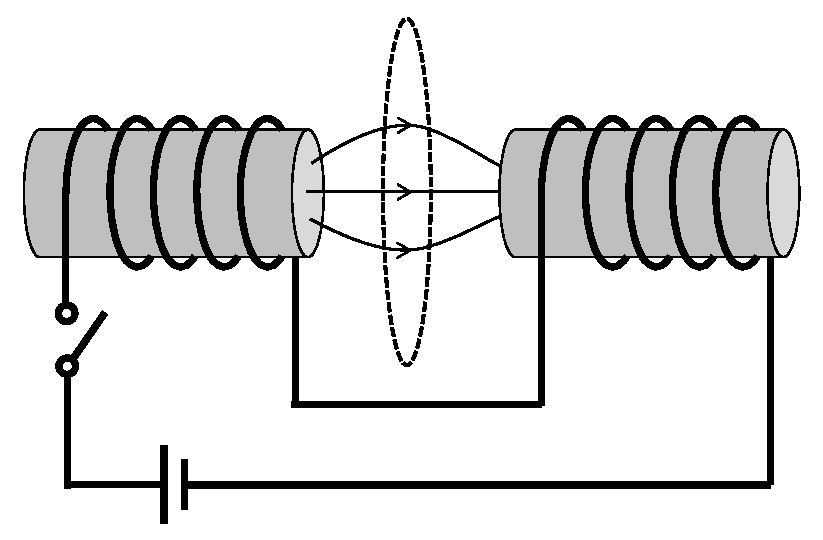
\includegraphics[width=0.4\textwidth]{deriving_em_waves/faradays_law.eps}
\vspace{-0.1in}
\end{center}

(f) In words, what does Faraday's law mean?

\begin{center}
Faraday sez: ``A changing \underline{\hspace{1in}} field induces a(n) \underline{\hspace{1in}} field.''
\end{center}
   
(g) Maxwell wondered if the reverse was also true: could a changing electric field also induce a magnetic field?  In the picture below, draw lines showing the electric field E as the capacitor charges up.  Is the electric field  increasing, decreasing, or staying the same?
\begin{center}
\vspace{-0.2in}
    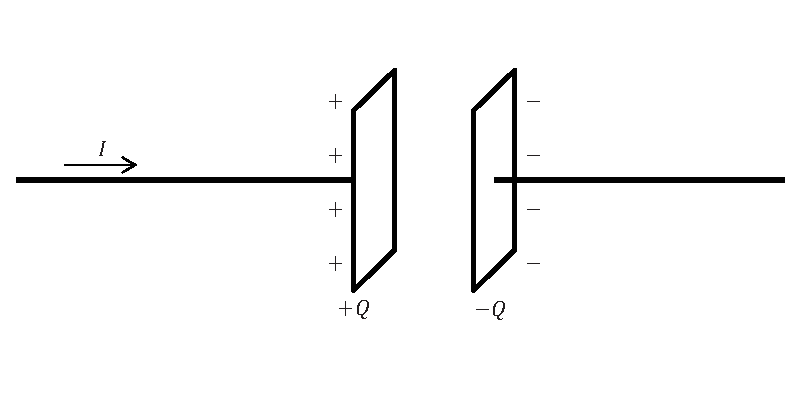
\includegraphics[width=0.6\textwidth]{deriving_em_waves/capacitor2.eps}
\end{center}

\pagebreak
\textbf{Activity 2: Help Maxwell Fix Up Ampere's Law!}

Maxwell decided to add a term involving $d\Phi_E)/dt$ to Amp\`ere's law, to account for magnetic field due to the change in electric field.
\begin{center}
\vspace{-0.2in}
    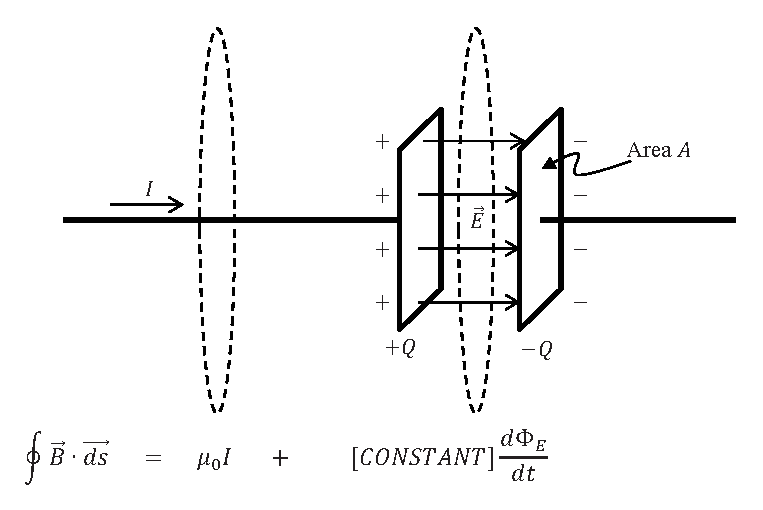
\includegraphics[width=0.55\textwidth]{deriving_em_waves/two_loops_with_equation.eps}
\vspace{-0.1in}
\end{center}

In this activity, you'll help Maxwell find the right value for the constant, so that $\vec B$ is the same around either of the dashed loops in the picture above.  This means finding the right value of the constant so that
\begin{displaymath}
\mu_0I = [CONSTANT] \frac{d\Phi_E}{dt}.
\end{displaymath}

(a) Rewrite the equation just above, writing the electric flux $\Phi_E$ in terms of the electric field $E$ and the area $A$.
\vspace{0.4in}

(b) What is the area $A$ you just used: the circular area of the loop, or the area of the capacitor plate?
\vspace{0.5in}

(c) If the plates have charge $+Q$ and $-Q$ on them, what is the electric field $E$ between the plates, in terms of $Q$ and $A$?
\vspace{0.6in}

(d) Rewrite your equation from part (a), in terms of $Q$ and $A$ instead of $E$.
\vspace{0.5in}

(e) What is the relationship between current $I$ and charge $Q$? (Hint: Perhaps something with a time derivative?)
\vspace{0.5in}

(f) Rewrite your equation from (d) in terms of $I$.
\vspace{0.5in}

(g) At this point it should be clear what that constant should be.  Rewrite the new, fixed-up version of Amp\`ere's law using the constant you've found.  Maxwell thanks you!  
\vspace{0.5in}

\pagebreak
\textbf{Activity 3} \newline
Maxwell must have been pretty excited to figure this out!  He already knew that a changing $\vec B$ could cause a $\vec E$, and now he knew that a changing $\vec E$ could cause a $\vec B$.  What if the two could keep causing each other?  Maybe a changing $\vec E$ could cause a $\vec B$, and then that could cause anothe $\vec E$, and so on, forever?  What would that look like? To find out, we'll look at the case of $\vec E$ and $\vec B$ shown in the figure below.

%Our goal now is to take the two equations we already have, Faraday's law and the newly fixed-up Amp\`ere's law, and see what kind of behavior they lead to in $\vec E$ and $\vec B$.  We'll do this by looking at a case where $\vec B$ is in the $z$ direction,and the electric field is along the $y$ axis, as shown in the figure below.  

\vspace{-0.1in}
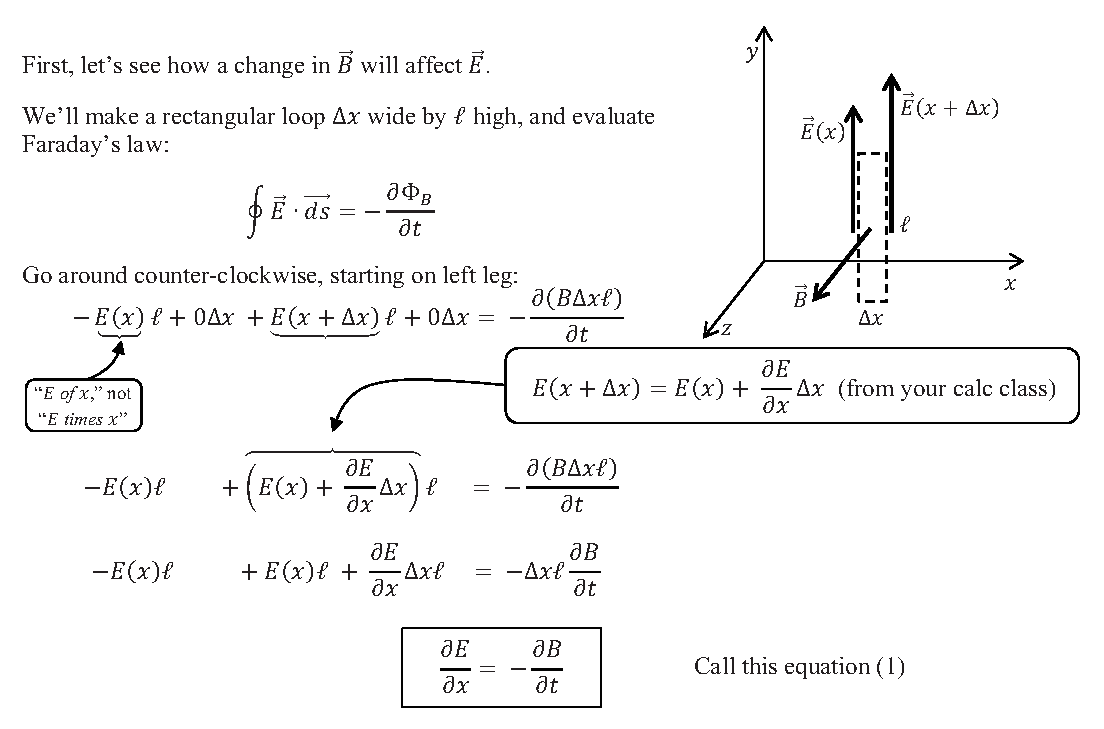
\includegraphics[width=0.9\textwidth]{deriving_em_waves/change_in_B.eps} \newline
\underline{\hspace{\textwidth}}
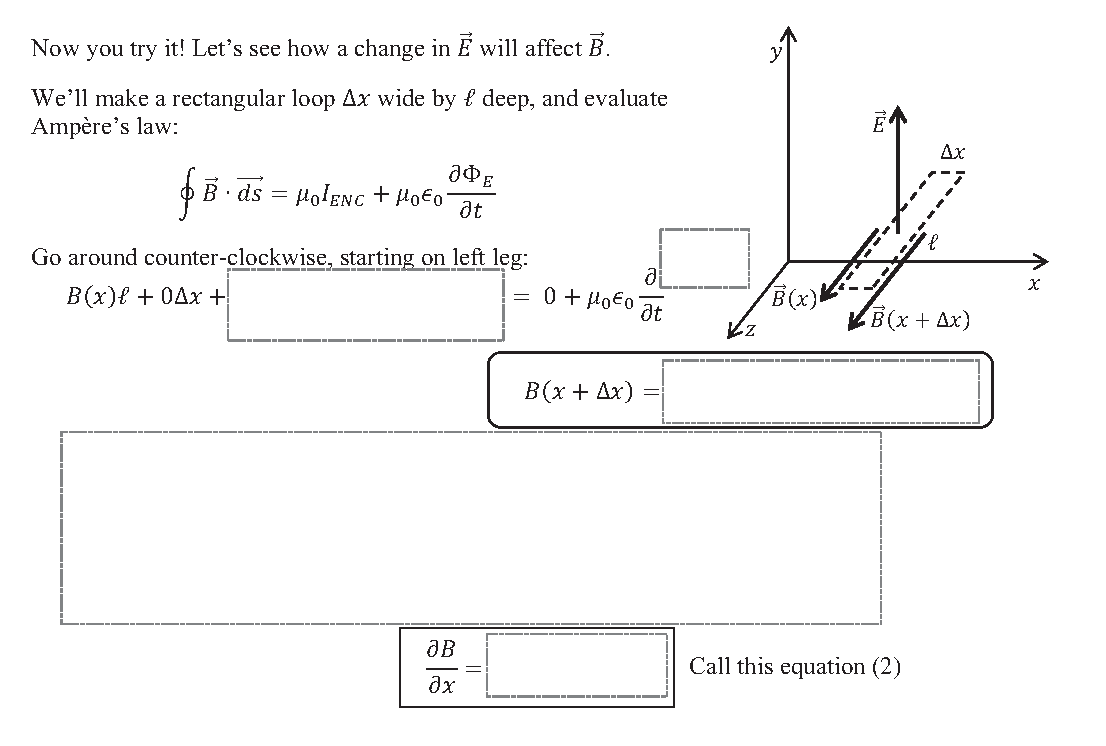
\includegraphics[width=0.9\textwidth]{deriving_em_waves/change_in_E_bw.eps}
\newpage

In equations (1) and (2) we now have equations that link time and spacial derivatives of $\vec E$ and $\vec B$ together.  Now, we'll do just a little more math to separate \textit{just} $\vec E$ in one equation, and \textit{just} $\vec B$ in another.  Again, we'll show you how to do it for one of them, then you'll do the other one.
\vspace{-0.2in}

\begin{center}
    \includegraphics[width=0.9\textwidth]{deriving_em_waves/separate_E_and_B.eps} 
 \end{center}
\vspace{-0.2in}

\textbf{Activity 4: What it all means}

You've seen equations like these before when you studied waves.  You know that in general, the equation for a one dimensional wave (like a wave on a string, for instance) is
\begin{displaymath}
\frac{\partial^2y(x,t)}{\partial t^2}= \frac{1}{v^2} \frac{\partial^2y(x,t)}{\partial x^2},
\end{displaymath}
where $v$ is the speed of the wave.  Maxwell knew this too, of course, and he was eager to find out how fast this new kind of wave traveled.

(a) Comparing the equations for $E$ and $B$ that you just derived with the wave equation above, what is the speed of the waves $\vec E(x,t)$ and $\vec B(x,t)$, in terms of $\mu_0$ and $\varepsilon_0$?
\vspace{0.5in}

(b)  The accepted values for $\mu_0$ and $\varepsilon_0$ are $\mu_0=4\pi \times 10^{-7}$ N$\cdot$s$^2$/C$^2$ and 
$\varepsilon_0=8.85 \times 10^{-12}$ C$^2$/N$\cdot $m$^2$.  Calculate a numerical value for the speed of the waves 
$\vec E(x,t)$ and $\vec B(x,t)$.
\vspace{0.5in}

(c) What else do you know that goes that fast?
\vspace{0.5in}

Maxwell knew that too!  And at the time, light was generally understood to be some kind of wave (due to interference and diffraction effects, for instance), but nobody could imagine what kind of wave it was, or what kind of thing was actually \textit{doing} the waving.  As Maxwell proclaimed, ``We can scarcely avoid the conclusion that light consists in the transverse undulations of the same medium which is the cause of electric and magnetic phenomena.''  Very quickly after that, Maxwell and other physicists were able to explain virtually every known property of optics in terms of electomagnetic phenomena.  In just over forty years, starting with  Hans Christian \/Orsted's discovery in 1819 that electric current could deflect a compass needle, physics had now completely unified the fields of magnetism, electricity, and optics into a single into a single theory.  





